\chapter{Progettazione e codifica}
\label{cap:progettazione-codifica}

\emph{In questo capitolo si descrive la progettazione e la codifica del sistema. Si inizia con una panoramica generale del sistema, per poi passare a una descrizione dettagliata delle varie componenti.}

\section{Introduzione}
Le fasi di un flusso di lavoro per l'Intelligent Document Processing (IDP) possono variare in base al caso d'uso specifico e ai requisiti aziendali, ma esistono alcune fasi comuni che sono generalmente presenti in qualsiasi processo IDP. Tali flussi di lavoro trovano applicazione in diversi ambiti, come l'elaborazione di moduli fiscali, reclami, note mediche, moduli di nuovi clienti, fatture, contratti legali, e molti altri documenti aziendali. 

Nel contesto del presente progetto, l'obiettivo è stato quello di rispondere alla richiesta dell'azienda ospitante di automatizzare la catalogazione e l'elaborazione delle email e dei relativi documenti allegati. A tal fine, è stato progettato un flusso di lavoro articolato in diverse fasi, ciascuna delle quali contribuisce a trasformare i documenti non strutturati in informazioni strutturate e utilizzabili. Le fasi individuate per il processo di elaborazione dei documenti dalle email sono le seguenti:

\begin{itemize}
  \item \textbf{Data Capture}: Questa fase riguarda l'estrazione degli allegati dalle email. I file vengono archiviati e aggregati in modo sicuro, garantendo la corretta gestione dei dati fin dal primo momento. Questo passaggio è cruciale per assicurare che tutte le informazioni necessarie siano raccolte e pronte per le fasi successive del processo.
  
  \item \textbf{Classification}: Una volta acquisiti, i documenti vengono classificati in base al loro contenuto. Questa fase consiste nell'assegnazione di ciascun documento a una specifica pipeline di elaborazione, in base alla tipologia di documento identificata. La corretta classificazione è fondamentale per assicurare che ogni documento segua il percorso di elaborazione più appropriato.

  \item \textbf{Extraction}: Durante questa fase, vengono estratte le informazioni aziendali rilevanti dai documenti. Si tratta di un processo automatizzato in cui i dati chiave vengono isolati e resi disponibili per ulteriori analisi. L'accuratezza di questa fase è determinante per il successo complessivo del flusso di lavoro, poiché influisce direttamente sulla qualità delle informazioni che verranno utilizzate.

  \item \textbf{Review and Validation}: Una volta estratte, le informazioni devono essere validate. In questa fase, vengono applicate regole di business per assicurare che i dati siano corretti e completi. Ove necessario, viene coinvolto un revisore umano per garantire la qualità delle informazioni estratte, riducendo il margine di errore e assicurando l'affidabilità del processo.

  \item \textbf{Storage}: Infine, le informazioni validate vengono salvate in un database aziendale. Questo passaggio è essenziale per garantire che i dati estratti siano facilmente accessibili per future consultazioni o analisi, completando così il ciclo di trasformazione dei documenti.
\end{itemize}

Questo flusso di lavoro, progettato per ottimizzare l'elaborazione automatizzata dei documenti, rappresenta un passo significativo verso l'efficienza operativa e la riduzione dei costi aziendali. Tale flusso è stato implementato utilizzando i servizi di AWS, in particolare AWS Lambda, Amazon Textract, Amazon Comprehend e Amazon DynamoDB. In particolare tramite AWS Step Functions è stato possibile orchestrare in modo efficiente le diverse fasi del processo, garantendo una gestione ottimale dei dati e una maggiore scalabilità.

\begin{figure}[h]
  \centering
  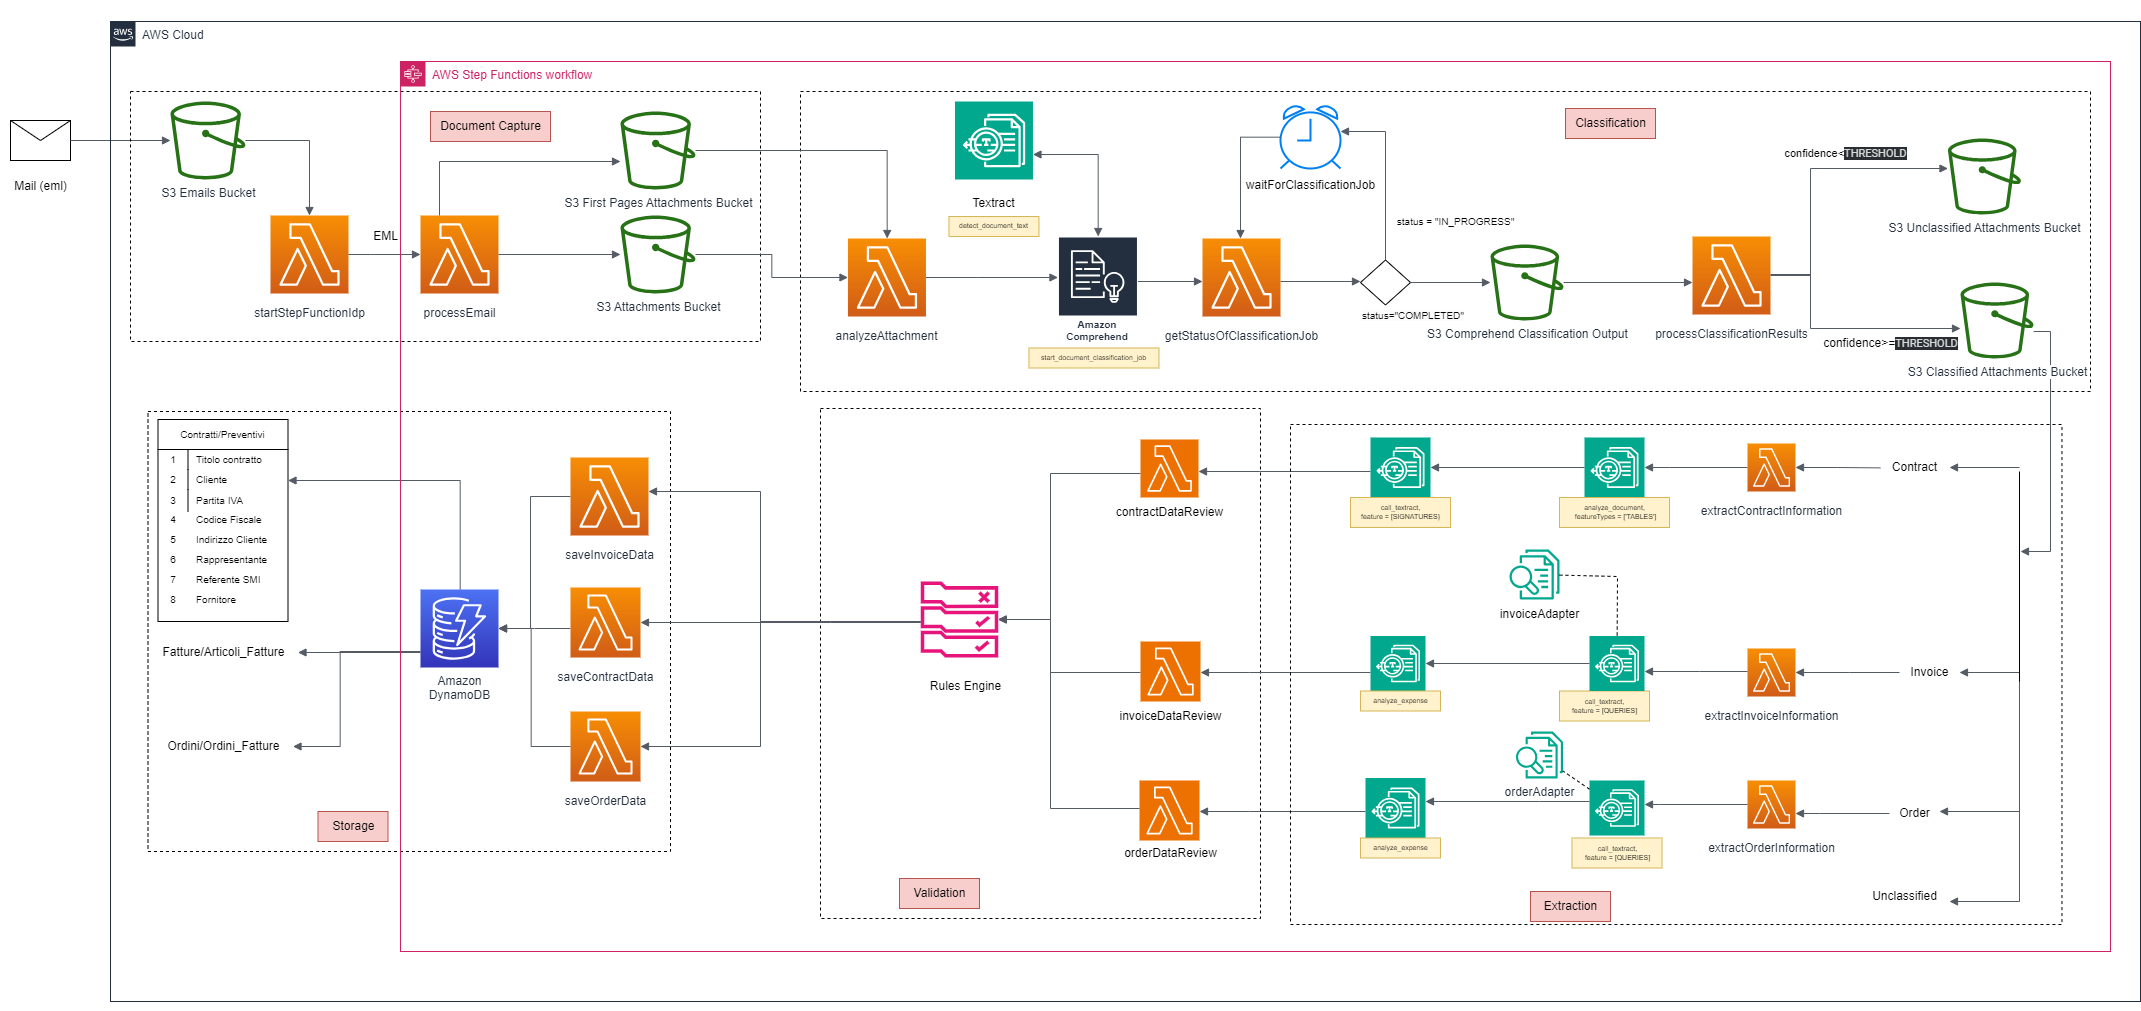
\includegraphics[width=1\textwidth]{img/design/classificatore_email.drawio.png}
  \caption{Flusso di lavoro per l'Intelligent Document Processing}
  \label{fig:IDP_workflow}
\end{figure}

Di seguito di visualizza la state machine "IdpStateMachine" nel dettaglio.

\begin{figure}[h]
  \centering
  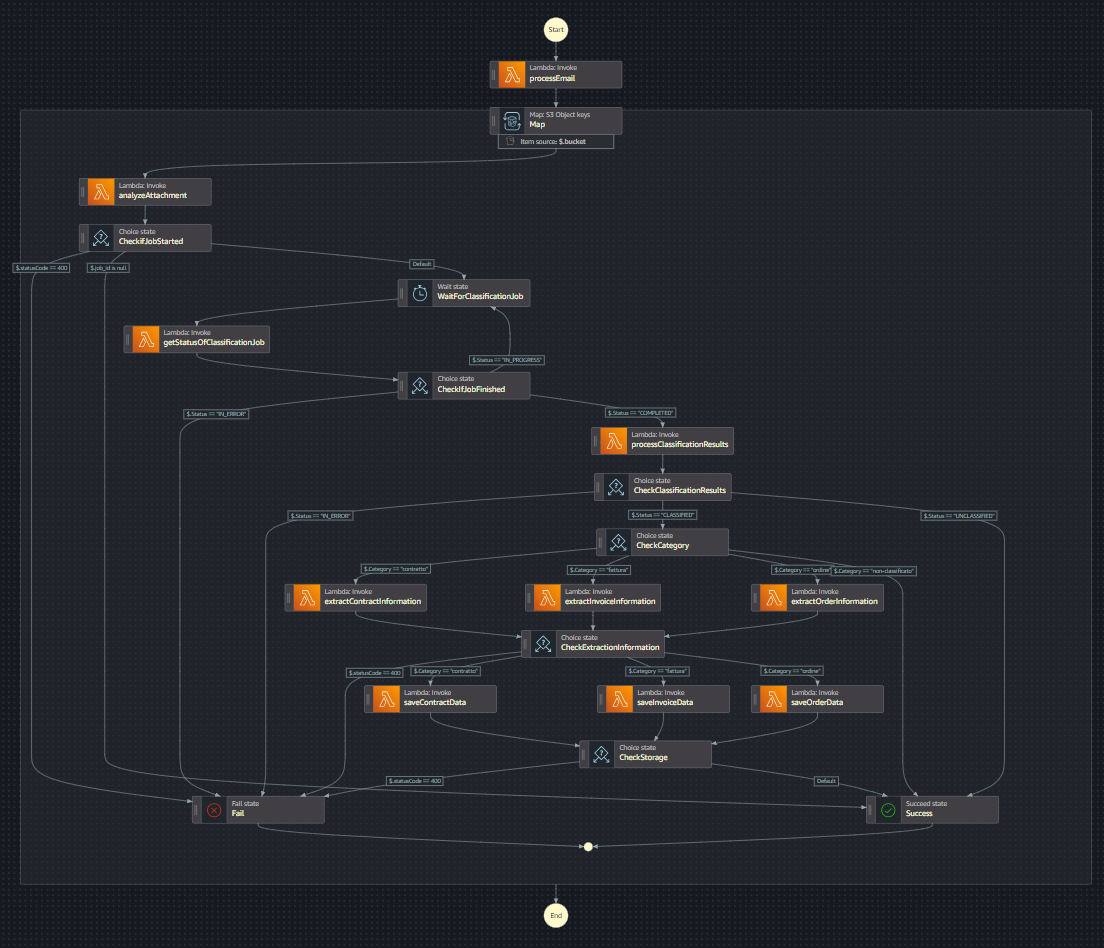
\includegraphics[width=1.1\textwidth]{img/design/IdpStateMachine.png}
  \caption{State Machine per l'Intelligent Document Processing}
  \label{fig:IDP_state_machine}
\end{figure}

\section{Architettura ad alto livello}
L'architettura proposta è stata concepita per classificare gli allegati delle email in quattro categorie principali: ordini, fatture, contratti e non classificato. Inoltre, il sistema è progettato per estrarre informazioni specifiche dai documenti appartenenti alle prime tre categorie, escludendo la categoria non classificato.

\section{Estrazione degli allegati}
\label{sec:estrazione-allegati}
Inizialmente, l'indicazione fornita dall'azienda richiedeva un'analisi del contenuto delle email, seguita da una classificazione basata sull'elaborazione del linguaggio naturale e sui metadati contenuti. Tuttavia, con il chiarimento delle categorie di interesse (ordini, fatture e contratti), ho deciso di concentrare l'attenzione sull'estrazione degli allegati presenti nelle email piuttosto che sul contenuto testuale delle stesse.

Questa scelta è giustificata dal fatto che i documenti di interesse per l'azienda sono spesso inclusi come allegati nelle email, rendendo l'estrazione degli allegati un approccio più diretto ed efficace. Inoltre, il contenuto delle email è spesso irrilevante o solo parzialmente utile per il processo di classificazione.

L'obiettivo principale di questa fase è quindi quello di ricavare gli allegati dalle email per poterli successivamente classificare e analizzare. Il processo è strutturato nelle seguenti fasi:

\begin{itemize}
    \item \textbf{Caricamento del file \texttt{.eml}}: Il processo inizia con il caricamento del file \texttt{.eml} nel bucket "S3 Emails Bucket", che funge da archivio per le email da analizzare.
    
    \item \textbf{Attivazione della funzione Lambda "StartStepFunctionIdp"}: L'inserimento del file \texttt{.eml} nel bucket attiva la funzione Lambda "StartStepFunctionIdp", la quale avvia l'esecuzione della state machine "IdpStateMachine" di AWS Step Functions. Questa state machine gestisce l'intero flusso di lavoro automatizzato.

    \item \textbf{Estrazione degli allegati}: La state machine avvia la funzione Lambda "processEmail", responsabile dell'estrazione degli allegati dalle email. Questa funzione è essenziale per isolare i documenti di interesse dal file \texttt{.eml}.

    \item \textbf{Caricamento degli allegati}: Una volta estratti, gli allegati vengono caricati nel bucket "S3 Attachments Bucket". In aggiunta, le prime pagine dei file PDF vengono salvate nel bucket "S3 First Pages Attachments Bucket". Gli allegati, che possono essere in vari formati (PDF, PNG, JPG, TXT, DOC, DOCX, ecc.), vengono archiviati in una cartella il cui nome corrisponde a quello della mail da cui provengono (file \texttt{.eml}).
\end{itemize}

Questa sequenza di operazioni permette di strutturare un flusso di lavoro chiaro e diretto, facilitando la successiva classificazione e analisi dei documenti estratti dalle email.

\section{Classificazione dei documenti}
\label{sec:classificazione-documenti}
Inizialmente, l'idea era di classificare le email in base al loro contenuto utilizzando modelli di \gls{mlg} offerti da Amazon SageMaker. Tuttavia, con il chiarimento delle categorie di interesse durante lo stage (ordini, fatture e contratti), si è deciso di focalizzarsi sull'estrazione e la classificazione degli allegati presenti nelle email, piuttosto che sul contenuto testuale delle stesse. Questo approccio ha semplificato significativamente il processo di classificazione, poiché i metadati (denominati anche \textit{features} nel contesto del machine learning) si riducono al semplice testo estratto dagli allegati.

La fase di classificazione degli allegati si articola nelle seguenti operazioni:

\begin{itemize}
    \item \textbf{Caricamento del file \texttt{.eml} e attivazione della pipeline}: Dopo l'estrazione degli allegati dalle email, descritta nella Sezione \ref{sec:estrazione-allegati}, i documenti vengono preparati per la classificazione. La funzione Lambda "analyzeAttachment" utilizza il classificatore di Amazon Comprehend denominato "document-classifier" per analizzare la prima pagina degli allegati. Il testo viene estratto tramite la funzione \texttt{detect\_document\_text} di Amazon Textract, che converte i contenuti dei documenti in un formato testuale adatto per l'analisi.

    \item \textbf{Salvataggio del risultato della classificazione}: I risultati del job di classificazione, composti da un file JSON che riporta la categoria assegnata e il relativo livello di confidenza, vengono salvati nel bucket "S3 Comprehend Classification Output". Questo passaggio consente di archiviare in modo strutturato i risultati, rendendoli disponibili per ulteriori elaborazioni.

    \item \textbf{Processamento dei risultati della classificazione}: Al termine del job di classificazione, la funzione Lambda "processClassificationResults" si attiva per salvare gli allegati classificati nei bucket appropriati. Se la confidenza del modello è superiore a una soglia (\textit{threshold}) predefinita, l'allegato viene salvato nel bucket "S3 Classified Attachments Bucket"; altrimenti, viene salvato nel bucket "S3 Unclassified Attachments Bucket". Gli allegati sono archiviati in cartelle che riportano la categoria di classificazione (ordine, fattura, contratto, non classificato). Questa organizzazione è fondamentale per facilitare la gestione e l'analisi successiva degli allegati, compresi quelli non classificati, che possono essere esaminati in dettaglio in un secondo momento.
\end{itemize}

Una precisazione importante riguarda la distinzione tra gli allegati salvati nel bucket "S3 Unclassified Attachments Bucket" e quelli salvati nel bucket "S3 Classified Attachments Bucket" all'interno della cartella "non classificato". Gli allegati presenti nel "S3 Unclassified Attachments Bucket" sono quelli per cui il livello di confidenza del modello è inferiore alla soglia predefinita. Al contrario, gli allegati presenti nella cartella "non classificato" del "S3 Classified Attachments Bucket" sono stati classificati con una confidenza superiore alla soglia, ma la categoria assegnata è comunque "non classificato", indicando una classificazione effettuata con un certo grado di sicurezza.

In questo contesto, l'utilizzo di Amazon Textract e Amazon Comprehend si è rivelato cruciale per l'accuratezza della classificazione. Sebbene in una fase iniziale fosse stato considerato l'uso del servizio Amazon Bedrock, in particolare con il modello Claude-3, questa opzione è stata successivamente scartata a favore di un modello personalizzato, ritenuto più adatto alle specifiche esigenze del progetto.
\subsection{Creazione del modello di classificazione personalizzato}
\label{subsec:training-modello}
La creazione di un modello di classificazione personalizzato con Amazon Comprehend richiede la disponibilità di un dataset ampio, significativo e bilanciato, capace di distinguere con precisione le categorie di interesse. È fondamentale che il dataset sia etichettato correttamente, in modo che ogni documento sia associato alla categoria di appartenenza.

Durante la fase di etichettatura, sono emerse alcune considerazioni chiave. I documenti da analizzare sono prevalentemente file PDF, spesso costituiti da scansioni. Per garantire coerenza nel processo di training, si è deciso di utilizzare esclusivamente documenti in formato PDF. Inoltre, è stato scelto di utilizzare unicamente le prime pagine di tali documenti per il training del modello. Questa scelta è stata motivata dal fatto che le prime pagine contengono generalmente le informazioni più rilevanti per la classificazione. Inoltre, considerando che il costo dell'analisi è proporzionale al numero di pagine, la riduzione del numero di pagine ha comportato una significativa riduzione dei costi operativi, soprattutto in documenti che possono arrivare fino a 100 pagine.

Tuttavia, queste scelte hanno anche portato a una riduzione della varietà dei dati utilizzati per il training, il che potrebbe potenzialmente introdurre \glsfirstoccur{\gls{biasg}} nel modello, limitando la sua capacità di generalizzare su nuovi dati. \\
Del modello personalizzato denominato "document-classifier" sono state create due versioni, ciascuna addestrata su dei dataset specifici. 
Per la prima versione del modello, denominata "document-classifier-version-1", sono stati utilizzati 47 documenti etichettati.\\
Per la seconda versione del modello, denominata "Comprehend-Generated-v1-
461f932", generata tramite il processo di Active Learning con Flywheel, sono stati utilizzati dei dataset di training di 56 documenti che si vanno ad aggiungere ai 47 documenti utilizzati per la versione precedente.
Per creare e distribuire il modello personalizzato, sono state seguite le seguenti fasi:
\begin{itemize}
    \item \textbf{Analisi del dataset}: È stata condotta un'analisi approfondita del dataset per valutare la distribuzione delle categorie e garantire un bilanciamento adeguato.
    \item \textbf{Preprocessing}: I dati sono stati preparati per il training, estratti i testi dai documenti PDF e organizzati in un file CSV.
    \item \textbf{Training}: Il modello personalizzato è stato addestrato utilizzando il file CSV creato in precedenza.
    \item \textbf{Valutazione}: Il modello è stato valutato utilizzando metriche standard per valutarne le prestazioni.
    \item \textbf{Test del modello}: Il modello è stato testato utilizzando nuovi documenti per verificare la sua capacità di generalizzazione.
\end{itemize}
\subsubsection{Analisi del dataset}
L'analisi del dataset è fondamentale per comprendere la distribuzione delle categorie e valutare l'adeguatezza dei dati per il training. Per i dataset utilizzati nelle varie iterazioni, le percentuali di distribuzione delle categorie (ordini, fatture, contratti e non classificato) sono state attentamente monitorate per garantire un bilanciamento adeguato.\\
Per il primo dataset di training, denominato "document-classifier-train", sono stati utilizzati 47 documenti etichettati, distribuiti nel modo seguente:
\begin{itemize}
    \item 25 contratti (53.19\%)
    \item 3 fatture (6.38\%)
    \item 5 ordini (10.64\%)
    \item 14 non classificati (29.79\%)
\end{itemize}
Per il secondo dataset di training, denominato "trainingFatture", sono stati utilizzati 26 documenti etichettati, distribuiti nel modo seguente:
\begin{itemize}
    \item 1 ordine (3.85\%)
    \item 25 fatture (96.15\%)
\end{itemize}
Per il terzo dataset di training, denominato "my-training-set", sono stati utilizzati 30 documenti etichettati, distribuiti nel modo seguente:
\begin{itemize}
    \item 10 fatture (33.33\%)
    \item 10 non classificati (33.33\%)
    \item 10 ordini (33.33\%)
\end{itemize}
Tali scelte sono state guidate dalla necessità di garantire un bilanciamento adeguato delle categorie, in modo da evitare che il modello sia influenzato da una distribuzione sbilanciata dei dati. Inoltre, è stato fondamentale assicurare che i documenti etichettati fossero rappresentativi delle categorie di interesse, in modo da garantire che il modello fosse in grado di generalizzare su nuovi dati.

\subsubsection{Preprocessing}
Il preprocessing dei dati è una fase critica del processo di addestramento. Le operazioni principali sono state:

\begin{itemize}
    \item Estrazione del testo tramite Amazon Textract: Il testo contenuto nelle prime pagine dei PDF è stato estratto utilizzando Amazon Textract.
    \item Creazione del file CSV: I dati estratti sono stati organizzati in un file CSV, con una colonna per la categoria di classificazione e una per il testo.
    \item Caricamento del file CSV: Il file di training CSV è stato caricato su Amazon S3 tramite Flywheel, per essere utilizzato nel processo di training.
\end{itemize}

\subsubsection{Training}
Durante la fase di training, il file CSV creato in precedenza è stato utilizzato per addestrare una nuova versione del classificatore personalizzato all'interno di Amazon Comprehend. Questo processo è stato gestito tramite il servizio Custom Classifier, che ha permesso di creare un modello ottimizzato per le esigenze specifiche del progetto.

\subsubsection{Valutazione}
La valutazione del modello è stata condotta utilizzando metriche standard, che hanno riportato i seguenti risultati per entrambe le versioni del modello:

\begin{itemize}
    \item Precision: 1.0
    \item Recall: 1.0
    \item F1: 1.0
    \item Accuracy: 1.0
    \item Micro precision: 1.0
    \item Micro recall: 1.0
    \item Micro F1: 1.0
\end{itemize}

Questi risultati indicano una performance ottimale del modello sulle classi di interesse.

\subsubsection{Test del modello}
Per testare il modello, è sufficiente caricare il file desiderato in un bucket S3 e avviare un job di classificazione. Il modello restituirà la categoria di classificazione assegnata al documento e il livello di confidenza associato, permettendo così una verifica immediata delle capacità del modello.

\subsubsection{Processo di Active Learning con Flywheel}
Per migliorare il modello nel tempo, è stato utilizzato il processo di \glsfirstoccur{\gls{activelearningg}} implementato tramite il servizio Flywheel di Amazon Comprehend. Questo approccio consente di iterare sul modello, migliorandolo progressivamente sulla base dei nuovi dati e delle prestazioni ottenute. Il processo segue questi passaggi:

\begin{itemize}
    \item Creazione di un dataset Flywheel: Si parte con la definizione di un dataset contenente i documenti etichettati, che verrà utilizzato per l'addestramento del modello.
    \item Inizializzazione di un'iterazione Flywheel: Viene avviata un'iterazione di Flywheel, durante la quale il modello viene addestrato sui dati disponibili.
    \item Attivazione del nuovo modello: Sulla base dei risultati dell'iterazione, viene deciso se attivare il nuovo modello. La decisione si basa su parametri predefiniti, come le metriche di precisione, recall e F1 score.
\end{itemize}




\section{Estrazione delle informazioni}
In questa fase l'obiettivo è l'estrazione delle informazioni associate a ciascuna categoria escludendo la categoria non classificato. A partire dai risultati di classificazione della fase precedente si è analizzato il metodo migliore per poter estrarre le informazioni ricercate dalle categorie di contratti, ordini e fatture. \\
Fondamentalmente sono stati analizzati diversi metodi utilizzando differenti servizi per aderire a tale scopo:
\begin{itemize}
    \item Comprehend custom entities
    \item Amazon Bedrock
    \item features di textract
\end{itemize}
Digressione sui vantaggi e svantaggi ... 
Alla fine si è optato per le seguenti opzioni:
\begin{itemize}
    \item Custom queries per le fatture 
    \item Custom queries per gli ordini 
    \item Analisi delle tabelle e dei form per i contratti 
\end{itemize}
C'è da sottolineare che per ogni informazione estratta viene anche riportata la percentuale di confidenza.
Il flusso per ogni categoria è il seguente:
\begin{itemize}
    \item Quando un file viene caricato nel bucket relativo ai documenti classificati tale azione scatena l'esecuzione di una lambda apposita per il tipo di documento 
    \item Al termine dell'esecuzione tali informazioni estratte vengono passate alla fase successiva 
\end{itemize}
\subsection{Estrazioni delle informazioni dai contratti}
Per tale fase essendo i contratti della stessa forma, (una tabella con le seguenti informazioni ...) si è optato per un'opzione poco costosa ma comunque efficiace. Tale soluzione consiste nell'identificare tale tabella ed estrarne i campi in base alla conoscenze note. 
\subsection{Estrazione delle informazioni dalle fatture e degli ordini}
Per tale fase si è pensato all'utilizzo di custom queries (adapter) di textract dato che tali documenti possiedono una struttura variabile. L'utilizzo di analisi delle fatture tramite la funzione apposita di textract è stata considerata ma poi scartata. Per gli ordini invece si è pensato di utilizzarla per ricavarne gli articoli in modo piu' diretto e sicuro. 
\section{Persistenza dei dati}
In questa fase l'obiettivo è far persistere i dati. La scelta è ricaduta su Amazon DynamoDB. Il flusso è il seguente:
\begin{itemize}
    \item Per ogni categoria (contratti, ordini, fatture) è creata una lambda, tale lambda salva i risultati delle informazioni estratte in DynamoDB nelle tabelle Ordini, Contratti, Fattura, Articoli\_Fatture, Articoli\_Ordini
\end{itemize}

\section{Analisi dei costi}
%\section{Tecnologie e strumenti}
%\label{sec:tecnologie-strumenti}
%
%Di seguito viene data una panoramica delle tecnologie e strumenti utilizzati.
%
%\subsection*{Tecnologia 1}
%Descrizione Tecnologia 1.
%
%\subsection*{Tecnologia 2}
%Descrizione Tecnologia 2
%
%\section{Ciclo di vita del software}
%\label{sec:ciclo-vita-software}
%
%\section{Progettazione}
%\label{sec:progettazione}
%
%\subsection{Namespace 1} %**************************
%Descrizione namespace 1.
%
%\begin{namespacedesc}
%    \classdesc{Classe 1}{Descrizione classe 1}
%    \classdesc{Classe 2}{Descrizione classe 2}
%\end{namespacedesc}
%
%
%\section{Design Pattern utilizzati}
%
%\section{Codifica}
